\section{Experiments}

We use the crypto data described above to train and test the performance of the different models. Due to computational limitations, we take the last 100k time steps with 90k time steps for training and the last 10k used as a test set. For LSTM and combined models, a sequence of 10 time-steps is taken together as inputs to the model. For GCN, a single frame and the 10-day lookback correlation matrix is used as inputs. Stochastic Gradient Descent (SGD) was used in parameter training. Hyperparameters were tuned manually to find a reasonable best-performing combination for LSTM and then used for training other models. The final combination was learning rate of 0.0001 and momentum of 0.9.

Our baseline model is a single-layer vanilla LSTM model with a hidden size of 14. Hidden and memory states are initialized to zero tensors. The embeddings at each of the 10 steps is flattened and fed through a final fully connected layer for predictions. Combined models use the baseline model and a single-layer GCN model that uses the above update and creates a 3-dimensional embedding that is then fed through a fully-connected layer to get the model's prediction.

\subsection{Combined Models}

We look at two ways of combining the component models: 1) additive and 2) sequential. The two methods are described below.

\textbf{Additive} In this combination scheme, the LSTM and GCN models make predictions independently using the given market-state input and correlation matrix. Their outputs are then combined via a weighted averaging where the weights on each model's outputs are constrained to sum to one and are also learnable parameters.

\textbf{Sequential} In this combination scheme, the market-state input is first passed through the LSTM. We take the last output of the LSTM as an embedding for the market state and use that with the correlation matrix as inputs to the GCN model which makes the final prediction. This is a special case of TGC as described above with correlation matrix as the adjacency matrix.

\subsection{Results}

Below is the training losses for our models.

\begin{figure}[H]
	\centering
	\begin{subfigure}{0.32\linewidth}
		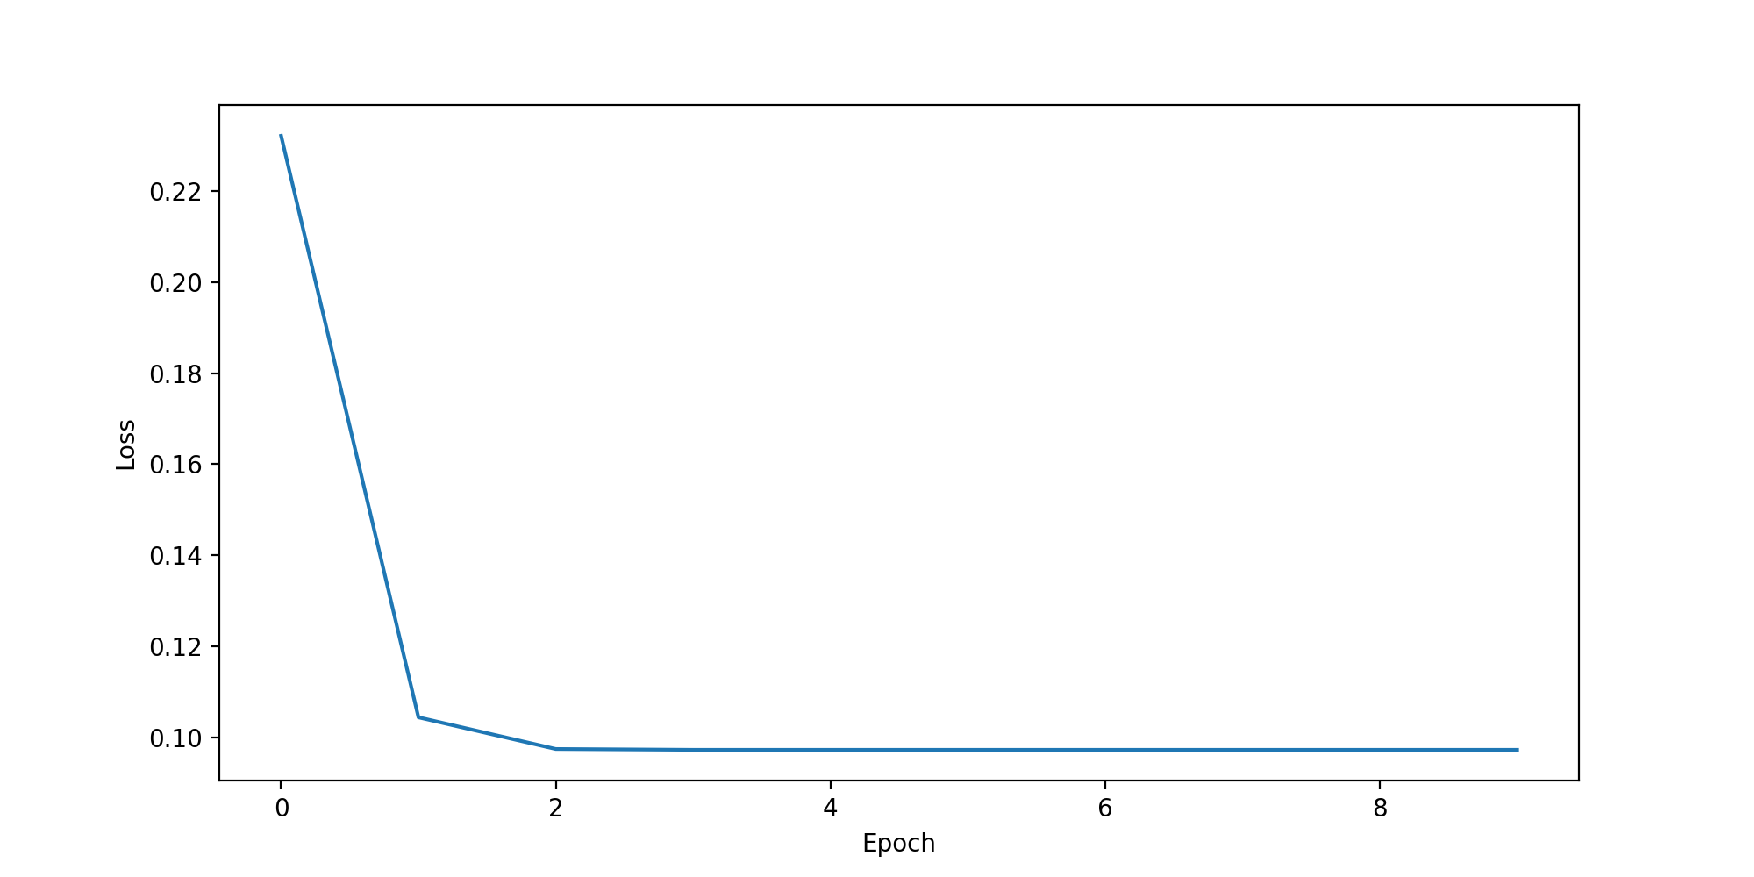
\includegraphics[width=\linewidth]{../../figures/vanilla_lstm_training_loss.pdf}
		\caption{LSTM}
	\end{subfigure}
	\begin{subfigure}{0.32\linewidth}
		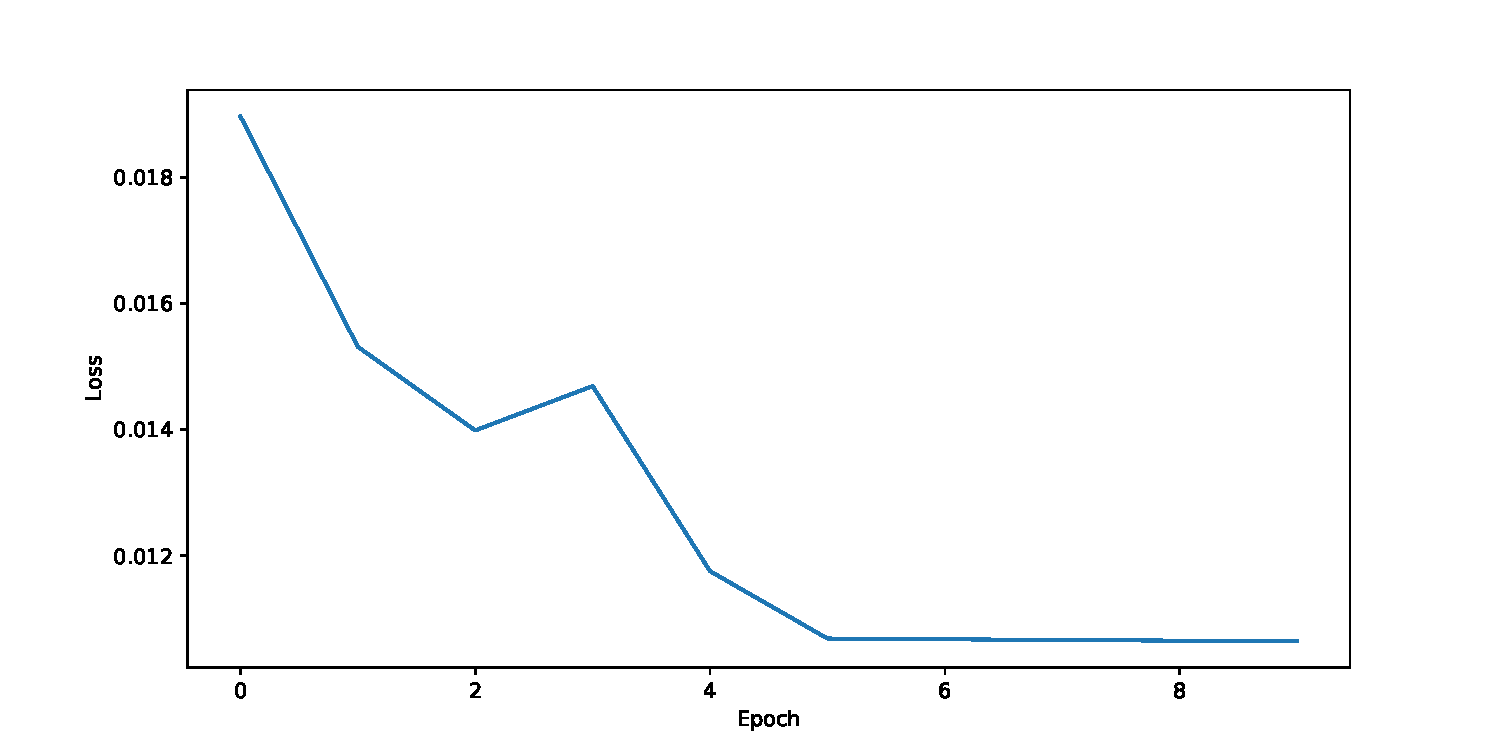
\includegraphics[width=\linewidth]{../../figures/additive_model_training_loss.pdf}
		\caption{Additive}
	\end{subfigure}
	\begin{subfigure}{0.32\linewidth}
		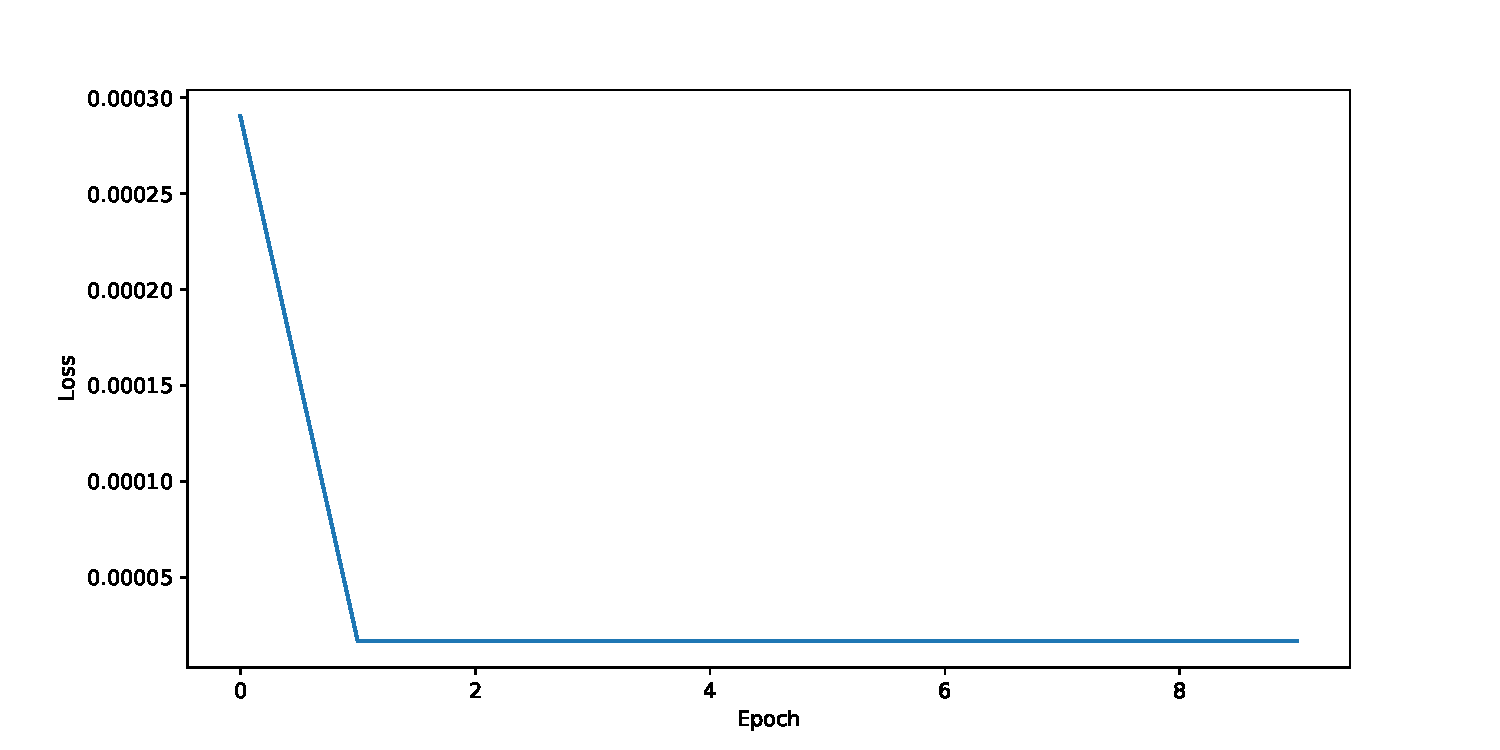
\includegraphics[width=\linewidth]{../../figures/sequential_model_training_loss.pdf}
		\caption{Sequential}
	\end{subfigure}
	\caption{Training loss of baseline LSTM model, additive model, and sequential model}
	\label{fig:lstm_loss}
\end{figure}

We see that with our given training scheme, all three models were able to reach saturation over the 10 epochs. Model performance was then tested on the held out validation set with the results shown in Table \ref{tab:results_summary}.

\begin{table}[H]
	\centering
	\begin{tabular}{|c|c|}
	\hline
	Model & MSE ($\times 10^{-4}$) \\
	\hline
	LSTM & 2.1831 \\
	Additive & 1.6396 \\
	Sequential & 0.1437 \\
	\hline
	\end{tabular}
	\caption{Average MSE on validation set}
	\label{tab:results_summary}
\end{table}